\Problem{Кубик Рубика}{1}{64}{inputN.txt}{outputN.txt}

Кубик Рубика~--- довольно сложная головоломка. Если вы никогда не собирали его, то скорее всего у вас не удастся это сделать
без сторонней помощи, хотя существуют люди, которые способны собирать данную головоломку в считанные секунды. К счастью у вас
есть компьютер, который скорее всего вам сильно поможет.

\begin{center}
	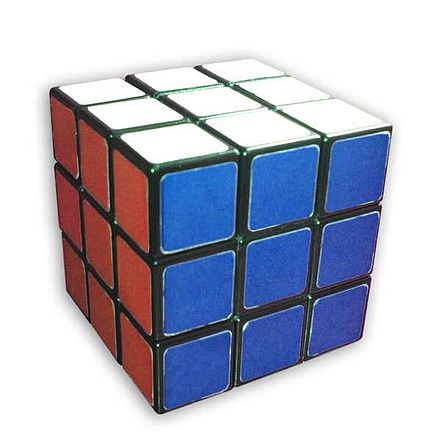
\includegraphics[width=200pt,natwidth=680,natheight=544]{tasks/rubiks/statements/images/solved.jpg}
\end{center}

Вам дана развертка Кубика Рубика. Нужно \textbf{попытаться} собрать его за любое разумное число ($\le 100\,000$) поворотов.

Повороты граней кубика описываются следующим образом:

\begin{itemize}
    \item \texttt{L}~--- поворот левой грани по часовой стрелке (если смотреть на нее);
    \item \texttt{R}~--- поворот правой грани по часовой стрелке (если смотреть на нее);
    \item \texttt{U}~--- поворот верхней грани по часовой стрелке (если смотреть на нее);
    \item \texttt{D}~--- поворот нижней грани по часовой стрелке (если смотреть на нее);
    \item \texttt{F}~--- поворот передней (фронтальной) грани по часовой стрелке (если смотреть на нее);
    \item \texttt{B}~--- поворот задней грани по часовой стрелке (если смотреть на нее);
\end{itemize}

Чтобы описать поворот против часовой стрелки, нужно после поворота добавить символ ``\textbf{'}''.

Развертка, которую вам дали имеет следующую структуру:

Первые три строки описывают цвета на верхней грани. В следующих трех строках идет описание граней по порядку:
передняя, правая, задняя, левая. В последних трех строках идет описание нижней грани. Верхняя грань имеет желтый цвет (\texttt{Y}),
нижняя~--- белый (\texttt{W}), левая~--- оранжевый (\texttt{O}), правая~--- красный (\texttt{R}), передняя~--- синий (\texttt{B}),
задняя~--- зеленый (\texttt{G}).

\Input
Вам дано 9 строк~--- описание развертки Кубика Рубика.

\Output
В единственной строке выведите повороты, которые нужны выполнить, чтобы \texttt{попытаться} собрать Кубик Рубика. Обратите внимание, что для получения
неполных баллов достаточно попытаться.

\Samples
\BeginTests
	\Test{tasks/rubiks/tests/samples}{01}{01.a}
\EndTests

\Scoring
Вы получите $10$ за тест, если Кубик Рубика окажется собраным. Если собрать не удалось, то вы получите $9 \cdot \frac{k - 6}{48}$ баллов, где $k$~--- количество
клеточек, которые совпадают по цвету со стороной.

\EndProblem
